\documentclass[1p]{elsarticle_modified}
%\bibliographystyle{elsarticle-num}

%\usepackage[colorlinks]{hyperref}
%\usepackage{abbrmath_seonhwa} %\Abb, \Ascr, \Acal ,\Abf, \Afrak
\usepackage{amsfonts}
\usepackage{amssymb}
\usepackage{amsmath}
\usepackage{amsthm}
\usepackage{scalefnt}
\usepackage{amsbsy}
\usepackage{kotex}
\usepackage{caption}
\usepackage{subfig}
\usepackage{color}
\usepackage{graphicx}
\usepackage{xcolor} %% white, black, red, green, blue, cyan, magenta, yellow
\usepackage{float}
\usepackage{setspace}
\usepackage{hyperref}

\usepackage{tikz}
\usetikzlibrary{arrows}

\usepackage{multirow}
\usepackage{array} % fixed length table
\usepackage{hhline}

%%%%%%%%%%%%%%%%%%%%%
\makeatletter
\renewcommand*\env@matrix[1][\arraystretch]{%
	\edef\arraystretch{#1}%
	\hskip -\arraycolsep
	\let\@ifnextchar\new@ifnextchar
	\array{*\c@MaxMatrixCols c}}
\makeatother %https://tex.stackexchange.com/questions/14071/how-can-i-increase-the-line-spacing-in-a-matrix
%%%%%%%%%%%%%%%

\usepackage[normalem]{ulem}

\newcommand{\msout}[1]{\ifmmode\text{\sout{\ensuremath{#1}}}\else\sout{#1}\fi}
%SOURCE: \msout is \stkout macro in https://tex.stackexchange.com/questions/20609/strikeout-in-math-mode

\newcommand{\cancel}[1]{
	\ifmmode
	{\color{red}\msout{#1}}
	\else
	{\color{red}\sout{#1}}
	\fi
}

\newcommand{\add}[1]{
	{\color{blue}\uwave{#1}}
}

\newcommand{\replace}[2]{
	\ifmmode
	{\color{red}\msout{#1}}{\color{blue}\uwave{#2}}
	\else
	{\color{red}\sout{#1}}{\color{blue}\uwave{#2}}
	\fi
}

\newcommand{\Sol}{\mathcal{S}} %segment
\newcommand{\D}{D} %diagram
\newcommand{\A}{\mathcal{A}} %arc


%%%%%%%%%%%%%%%%%%%%%%%%%%%%%5 test

\def\sl{\operatorname{\textup{SL}}(2,\Cbb)}
\def\psl{\operatorname{\textup{PSL}}(2,\Cbb)}
\def\quan{\mkern 1mu \triangleright \mkern 1mu}

\theoremstyle{definition}
\newtheorem{thm}{Theorem}[section]
\newtheorem{prop}[thm]{Proposition}
\newtheorem{lem}[thm]{Lemma}
\newtheorem{ques}[thm]{Question}
\newtheorem{cor}[thm]{Corollary}
\newtheorem{defn}[thm]{Definition}
\newtheorem{exam}[thm]{Example}
\newtheorem{rmk}[thm]{Remark}
\newtheorem{alg}[thm]{Algorithm}

\newcommand{\I}{\sqrt{-1}}
\begin{document}

%\begin{frontmatter}
%
%\title{Boundary parabolic representations of knots up to 8 crossings}
%
%%% Group authors per affiliation:
%\author{Yunhi Cho} 
%\address{Department of Mathematics, University of Seoul, Seoul, Korea}
%\ead{yhcho@uos.ac.kr}
%
%
%\author{Seonhwa Kim} %\fnref{s_kim}}
%\address{Center for Geometry and Physics, Institute for Basic Science, Pohang, 37673, Korea}
%\ead{ryeona17@ibs.re.kr}
%
%\author{Hyuk Kim}
%\address{Department of Mathematical Sciences, Seoul National University, Seoul 08826, Korea}
%\ead{hyukkim@snu.ac.kr}
%
%\author{Seokbeom Yoon}
%\address{Department of Mathematical Sciences, Seoul National University, Seoul, 08826,  Korea}
%\ead{sbyoon15@snu.ac.kr}
%
%\begin{abstract}
%We find all boundary parabolic representation of knots up to 8 crossings.
%
%\end{abstract}
%\begin{keyword}
%    \MSC[2010] 57M25 
%\end{keyword}
%
%\end{frontmatter}

%\linenumbers
%\tableofcontents
%
\newcommand\colored[1]{\textcolor{white}{\rule[-0.35ex]{0.8em}{1.4ex}}\kern-0.8em\color{red} #1}%
%\newcommand\colored[1]{\textcolor{white}{ #1}\kern-2.17ex	\textcolor{white}{ #1}\kern-1.81ex	\textcolor{white}{ #1}\kern-2.15ex\color{red}#1	}

{\Large $\underline{12a_{0607}~(K12a_{0607})}$}

\setlength{\tabcolsep}{10pt}
\renewcommand{\arraystretch}{1.6}
\vspace{1cm}\begin{tabular}{m{100pt}>{\centering\arraybackslash}m{274pt}}
\multirow{5}{120pt}{
	\centering
	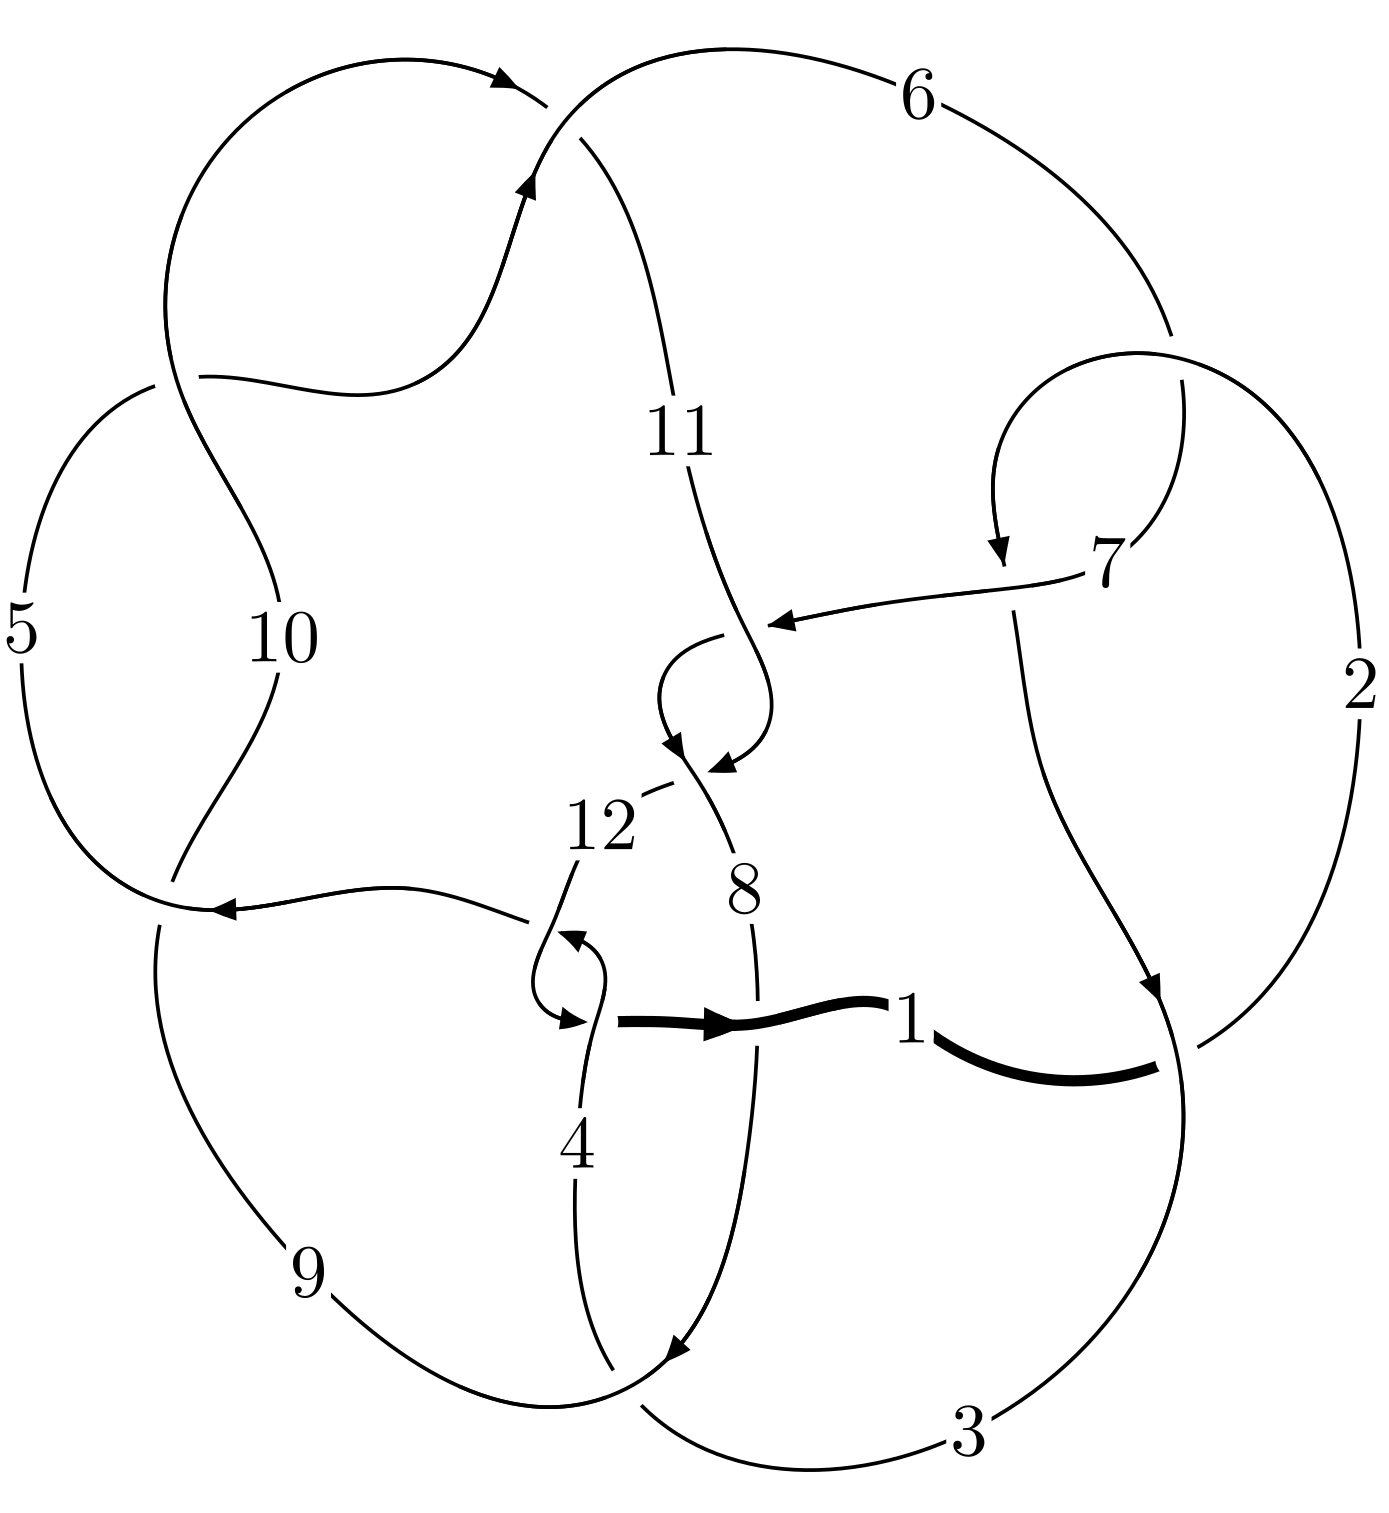
\includegraphics[width=112pt]{../../../GIT/diagram.site/Diagrams/png/1408_12a_0607.png}\\
\ \ \ A knot diagram\footnotemark}&
\allowdisplaybreaks
\textbf{Linearized knot diagam} \\
\cline{2-2}
 &
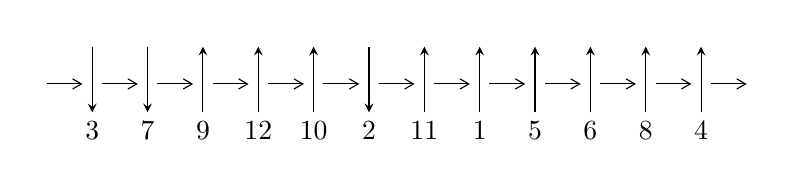
\begin{tikzpicture}[x=20pt, y=17pt]
	% nodes
	\node (C0) at (0, 0) {};
	\node (C1) at (1, 0) {};
	\node (C1U) at (1, +1) {};
	\node (C1D) at (1, -1) {3};

	\node (C2) at (2, 0) {};
	\node (C2U) at (2, +1) {};
	\node (C2D) at (2, -1) {7};

	\node (C3) at (3, 0) {};
	\node (C3U) at (3, +1) {};
	\node (C3D) at (3, -1) {9};

	\node (C4) at (4, 0) {};
	\node (C4U) at (4, +1) {};
	\node (C4D) at (4, -1) {12};

	\node (C5) at (5, 0) {};
	\node (C5U) at (5, +1) {};
	\node (C5D) at (5, -1) {10};

	\node (C6) at (6, 0) {};
	\node (C6U) at (6, +1) {};
	\node (C6D) at (6, -1) {2};

	\node (C7) at (7, 0) {};
	\node (C7U) at (7, +1) {};
	\node (C7D) at (7, -1) {11};

	\node (C8) at (8, 0) {};
	\node (C8U) at (8, +1) {};
	\node (C8D) at (8, -1) {1};

	\node (C9) at (9, 0) {};
	\node (C9U) at (9, +1) {};
	\node (C9D) at (9, -1) {5};

	\node (C10) at (10, 0) {};
	\node (C10U) at (10, +1) {};
	\node (C10D) at (10, -1) {6};

	\node (C11) at (11, 0) {};
	\node (C11U) at (11, +1) {};
	\node (C11D) at (11, -1) {8};

	\node (C12) at (12, 0) {};
	\node (C12U) at (12, +1) {};
	\node (C12D) at (12, -1) {4};
	\node (C13) at (13, 0) {};

	% arrows
	\draw[->,>={angle 60}]
	(C0) edge (C1) (C1) edge (C2) (C2) edge (C3) (C3) edge (C4) (C4) edge (C5) (C5) edge (C6) (C6) edge (C7) (C7) edge (C8) (C8) edge (C9) (C9) edge (C10) (C10) edge (C11) (C11) edge (C12) (C12) edge (C13) ;	\draw[->,>=stealth]
	(C1U) edge (C1D) (C2U) edge (C2D) (C3D) edge (C3U) (C4D) edge (C4U) (C5D) edge (C5U) (C6U) edge (C6D) (C7D) edge (C7U) (C8D) edge (C8U) (C9D) edge (C9U) (C10D) edge (C10U) (C11D) edge (C11U) (C12D) edge (C12U) ;
	\end{tikzpicture} \\
\hhline{~~} \\& 
\textbf{Solving Sequence} \\ \cline{2-2} 
 &
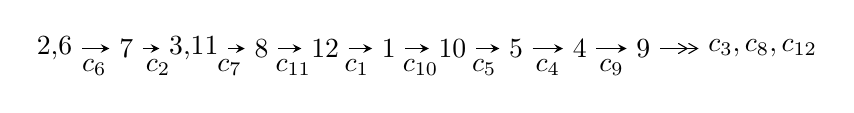
\begin{tikzpicture}[x=23pt, y=7pt]
	% node
	\node (A0) at (-1/8, 0) {2,6};
	\node (A1) at (1, 0) {7};
	\node (A2) at (33/16, 0) {3,11};
	\node (A3) at (25/8, 0) {8};
	\node (A4) at (33/8, 0) {12};
	\node (A5) at (41/8, 0) {1};
	\node (A6) at (49/8, 0) {10};
	\node (A7) at (57/8, 0) {5};
	\node (A8) at (65/8, 0) {4};
	\node (A9) at (73/8, 0) {9};
	\node (C1) at (1/2, -1) {$c_{6}$};
	\node (C2) at (3/2, -1) {$c_{2}$};
	\node (C3) at (21/8, -1) {$c_{7}$};
	\node (C4) at (29/8, -1) {$c_{11}$};
	\node (C5) at (37/8, -1) {$c_{1}$};
	\node (C6) at (45/8, -1) {$c_{10}$};
	\node (C7) at (53/8, -1) {$c_{5}$};
	\node (C8) at (61/8, -1) {$c_{4}$};
	\node (C9) at (69/8, -1) {$c_{9}$};
	\node (A10) at (11, 0) {$c_{3},c_{8},c_{12}$};

	% edge
	\draw[->,>=stealth]	
	(A0) edge (A1) (A1) edge (A2) (A2) edge (A3) (A3) edge (A4) (A4) edge (A5) (A5) edge (A6) (A6) edge (A7) (A7) edge (A8) (A8) edge (A9) ;
	\draw[->>,>={angle 60}]	
	(A9) edge (A10);
\end{tikzpicture} \\ 

\end{tabular} \\

\footnotetext{
The image of knot diagram is generated by the software ``\textbf{Draw programme}" developed by Andrew Bartholomew(\url{http://www.layer8.co.uk/maths/draw/index.htm\#Running-draw}), where we modified some parts for our purpose(\url{https://github.com/CATsTAILs/LinksPainter}).
}\phantom \\ \newline 
\centering \textbf{Ideals for irreducible components\footnotemark of $X_{\text{par}}$} 
 
\begin{align*}
I^u_{1}&=\langle 
-2.26145\times10^{231} u^{113}+5.03095\times10^{231} u^{112}+\cdots+2.30777\times10^{232} b-4.08208\times10^{232},\\
\phantom{I^u_{1}}&\phantom{= \langle  }1.92889\times10^{232} u^{113}-6.36228\times10^{232} u^{112}+\cdots+2.30777\times10^{232} a-1.06029\times10^{233},\;u^{114}-3 u^{113}+\cdots-9 u+1\rangle \\
I^u_{2}&=\langle 
-21 u^{27}+10 u^{26}+\cdots+2 b-19,\;-70 u^{27}+54 u^{26}+\cdots+2 a-63,\;u^{28}-7 u^{26}+\cdots-7 u^2+1\rangle \\
\\
\end{align*}
\raggedright * 2 irreducible components of $\dim_{\mathbb{C}}=0$, with total 142 representations.\\
\footnotetext{All coefficients of polynomials are rational numbers. But the coefficients are sometimes approximated in decimal forms when there is not enough margin.}
\newpage
\renewcommand{\arraystretch}{1}
\centering \section*{I. $I^u_{1}= \langle -2.26\times10^{231} u^{113}+5.03\times10^{231} u^{112}+\cdots+2.31\times10^{232} b-4.08\times10^{232},\;1.93\times10^{232} u^{113}-6.36\times10^{232} u^{112}+\cdots+2.31\times10^{232} a-1.06\times10^{233},\;u^{114}-3 u^{113}+\cdots-9 u+1 \rangle$}
\flushleft \textbf{(i) Arc colorings}\\
\begin{tabular}{m{7pt} m{180pt} m{7pt} m{180pt} }
\flushright $a_{2}=$&$\begin{pmatrix}0\\u\end{pmatrix}$ \\
\flushright $a_{6}=$&$\begin{pmatrix}1\\0\end{pmatrix}$ \\
\flushright $a_{7}=$&$\begin{pmatrix}1\\u^2\end{pmatrix}$ \\
\flushright $a_{3}=$&$\begin{pmatrix}- u\\- u^3+u\end{pmatrix}$ \\
\flushright $a_{11}=$&$\begin{pmatrix}-0.835823 u^{113}+2.75689 u^{112}+\cdots+12.9197 u+4.59444\\0.0979929 u^{113}-0.218000 u^{112}+\cdots-1.42503 u+1.76884\end{pmatrix}$ \\
\flushright $a_{8}=$&$\begin{pmatrix}-0.140571 u^{113}+0.865203 u^{112}+\cdots+20.0913 u-9.45803\\0.0539117 u^{113}+0.0112822 u^{112}+\cdots+4.42174 u-3.00291\end{pmatrix}$ \\
\flushright $a_{12}=$&$\begin{pmatrix}-1.04769 u^{113}+3.21627 u^{112}+\cdots+12.2084 u-6.84623\\-0.162523 u^{113}+0.434835 u^{112}+\cdots-2.74906 u-2.14289\end{pmatrix}$ \\
\flushright $a_{1}=$&$\begin{pmatrix}u^3\\u^5- u^3+u\end{pmatrix}$ \\
\flushright $a_{10}=$&$\begin{pmatrix}-0.933816 u^{113}+2.97489 u^{112}+\cdots+14.3447 u+2.82560\\0.0979929 u^{113}-0.218000 u^{112}+\cdots-1.42503 u+1.76884\end{pmatrix}$ \\
\flushright $a_{5}=$&$\begin{pmatrix}-0.603142 u^{113}+1.89788 u^{112}+\cdots+5.83444 u+6.88505\\-0.0853653 u^{113}+0.0879853 u^{112}+\cdots-4.45011 u+3.08256\end{pmatrix}$ \\
\flushright $a_{4}=$&$\begin{pmatrix}0.240716 u^{113}-0.351628 u^{112}+\cdots+104.338 u-3.46261\\-0.129888 u^{113}+0.442143 u^{112}+\cdots+34.0231 u-0.816845\end{pmatrix}$ \\
\flushright $a_{9}=$&$\begin{pmatrix}-0.127045 u^{113}+0.763359 u^{112}+\cdots+19.0070 u-9.34243\\0.0914259 u^{113}-0.176272 u^{112}+\cdots+1.60745 u-2.70612\end{pmatrix}$\\&\end{tabular}
\flushleft \textbf{(ii) Obstruction class $= -1$}\\~\\
\flushleft \textbf{(iii) Cusp Shapes $= -2.28402 u^{113}+7.67069 u^{112}+\cdots+6.89091 u+6.29754$}\\~\\
\newpage\renewcommand{\arraystretch}{1}
\flushleft \textbf{(iv) u-Polynomials at the component}\newline \\
\begin{tabular}{m{50pt}|m{274pt}}
Crossings & \hspace{64pt}u-Polynomials at each crossing \\
\hline $$\begin{aligned}c_{1}\end{aligned}$$&$\begin{aligned}
&u^{114}+41 u^{113}+\cdots-29 u+1
\end{aligned}$\\
\hline $$\begin{aligned}c_{2},c_{6}\end{aligned}$$&$\begin{aligned}
&u^{114}-3 u^{113}+\cdots-9 u+1
\end{aligned}$\\
\hline $$\begin{aligned}c_{3}\end{aligned}$$&$\begin{aligned}
&u^{114}- u^{113}+\cdots+621 u-135
\end{aligned}$\\
\hline $$\begin{aligned}c_{4},c_{12}\end{aligned}$$&$\begin{aligned}
&u^{114}+5 u^{113}+\cdots-4 u+1
\end{aligned}$\\
\hline $$\begin{aligned}c_{5},c_{9},c_{10}\end{aligned}$$&$\begin{aligned}
&u^{114}+u^{113}+\cdots-18 u-19
\end{aligned}$\\
\hline $$\begin{aligned}c_{7},c_{11}\end{aligned}$$&$\begin{aligned}
&u^{114}+3 u^{113}+\cdots+9623 u-24763
\end{aligned}$\\
\hline $$\begin{aligned}c_{8}\end{aligned}$$&$\begin{aligned}
&u^{114}+2 u^{113}+\cdots+3 u-1
\end{aligned}$\\
\hline
\end{tabular}\\~\\
\newpage\renewcommand{\arraystretch}{1}
\flushleft \textbf{(v) Riley Polynomials at the component}\newline \\
\begin{tabular}{m{50pt}|m{274pt}}
Crossings & \hspace{64pt}Riley Polynomials at each crossing \\
\hline $$\begin{aligned}c_{1}\end{aligned}$$&$\begin{aligned}
&y^{114}+75 y^{113}+\cdots+6061 y+1
\end{aligned}$\\
\hline $$\begin{aligned}c_{2},c_{6}\end{aligned}$$&$\begin{aligned}
&y^{114}-41 y^{113}+\cdots+29 y+1
\end{aligned}$\\
\hline $$\begin{aligned}c_{3}\end{aligned}$$&$\begin{aligned}
&y^{114}-11 y^{113}+\cdots-978561 y+18225
\end{aligned}$\\
\hline $$\begin{aligned}c_{4},c_{12}\end{aligned}$$&$\begin{aligned}
&y^{114}+65 y^{113}+\cdots-44 y+1
\end{aligned}$\\
\hline $$\begin{aligned}c_{5},c_{9},c_{10}\end{aligned}$$&$\begin{aligned}
&y^{114}-123 y^{113}+\cdots+38854 y+361
\end{aligned}$\\
\hline $$\begin{aligned}c_{7},c_{11}\end{aligned}$$&$\begin{aligned}
&y^{114}-99 y^{113}+\cdots-42189999285 y+613206169
\end{aligned}$\\
\hline $$\begin{aligned}c_{8}\end{aligned}$$&$\begin{aligned}
&y^{114}-8 y^{113}+\cdots-169 y+1
\end{aligned}$\\
\hline
\end{tabular}\\~\\
\newpage\flushleft \textbf{(vi) Complex Volumes and Cusp Shapes}
$$\begin{array}{c|c|c}  
\text{Solutions to }I^u_{1}& \I (\text{vol} + \sqrt{-1}CS) & \text{Cusp shape}\\
 \hline 
\begin{aligned}
u &= -0.687146 + 0.735720 I \\
a &= -0.711893 - 0.154086 I \\
b &= \phantom{-}1.62059 - 0.07956 I\end{aligned}
 & \phantom{-}10.22650 - 1.77188 I & \phantom{-0.000000 } 0 \\ \hline\begin{aligned}
u &= -0.687146 - 0.735720 I \\
a &= -0.711893 + 0.154086 I \\
b &= \phantom{-}1.62059 + 0.07956 I\end{aligned}
 & \phantom{-}10.22650 + 1.77188 I & \phantom{-0.000000 } 0 \\ \hline\begin{aligned}
u &= -0.416841 + 0.898796 I \\
a &= \phantom{-}0.593965 - 0.281830 I \\
b &= \phantom{-}0.419388 + 0.044804 I\end{aligned}
 & \phantom{-}1.18254 + 4.12227 I & \phantom{-0.000000 } 0 \\ \hline\begin{aligned}
u &= -0.416841 - 0.898796 I \\
a &= \phantom{-}0.593965 + 0.281830 I \\
b &= \phantom{-}0.419388 - 0.044804 I\end{aligned}
 & \phantom{-}1.18254 - 4.12227 I & \phantom{-0.000000 } 0 \\ \hline\begin{aligned}
u &= \phantom{-}0.656531 + 0.741360 I \\
a &= -0.303134 + 0.456349 I \\
b &= \phantom{-}1.52215 + 0.05789 I\end{aligned}
 & \phantom{-}9.90297 - 1.32162 I & \phantom{-0.000000 } 0 \\ \hline\begin{aligned}
u &= \phantom{-}0.656531 - 0.741360 I \\
a &= -0.303134 - 0.456349 I \\
b &= \phantom{-}1.52215 - 0.05789 I\end{aligned}
 & \phantom{-}9.90297 + 1.32162 I & \phantom{-0.000000 } 0 \\ \hline\begin{aligned}
u &= \phantom{-}1.022400 + 0.102373 I \\
a &= \phantom{-}0.09858 + 1.51788 I \\
b &= \phantom{-}0.197689 + 0.736964 I\end{aligned}
 & -5.82932 + 1.67100 I & \phantom{-0.000000 } 0 \\ \hline\begin{aligned}
u &= \phantom{-}1.022400 - 0.102373 I \\
a &= \phantom{-}0.09858 - 1.51788 I \\
b &= \phantom{-}0.197689 - 0.736964 I\end{aligned}
 & -5.82932 - 1.67100 I & \phantom{-0.000000 } 0 \\ \hline\begin{aligned}
u &= -0.966026 + 0.044927 I \\
a &= -0.86533 - 1.32827 I \\
b &= -1.349860 - 0.318487 I\end{aligned}
 & -0.96786 + 5.47578 I & \phantom{-0.000000 } 0 \\ \hline\begin{aligned}
u &= -0.966026 - 0.044927 I \\
a &= -0.86533 + 1.32827 I \\
b &= -1.349860 + 0.318487 I\end{aligned}
 & -0.96786 - 5.47578 I & \phantom{-0.000000 } 0\\
 \hline 
 \end{array}$$\newpage$$\begin{array}{c|c|c}  
\text{Solutions to }I^u_{1}& \I (\text{vol} + \sqrt{-1}CS) & \text{Cusp shape}\\
 \hline 
\begin{aligned}
u &= \phantom{-}0.674987 + 0.789459 I \\
a &= \phantom{-}0.149508 - 0.108550 I \\
b &= \phantom{-}1.64038 + 0.36093 I\end{aligned}
 & \phantom{-}10.44150 + 2.65068 I & \phantom{-0.000000 } 0 \\ \hline\begin{aligned}
u &= \phantom{-}0.674987 - 0.789459 I \\
a &= \phantom{-}0.149508 + 0.108550 I \\
b &= \phantom{-}1.64038 - 0.36093 I\end{aligned}
 & \phantom{-}10.44150 - 2.65068 I & \phantom{-0.000000 } 0 \\ \hline\begin{aligned}
u &= -0.694806 + 0.781406 I \\
a &= -0.085877 + 0.391899 I \\
b &= \phantom{-}1.76063 - 0.18976 I\end{aligned}
 & \phantom{-}10.74210 + 1.01393 I & \phantom{-0.000000 } 0 \\ \hline\begin{aligned}
u &= -0.694806 - 0.781406 I \\
a &= -0.085877 - 0.391899 I \\
b &= \phantom{-}1.76063 + 0.18976 I\end{aligned}
 & \phantom{-}10.74210 - 1.01393 I & \phantom{-0.000000 } 0 \\ \hline\begin{aligned}
u &= -0.663472 + 0.826356 I \\
a &= \phantom{-}0.572692 - 0.380758 I \\
b &= \phantom{-}0.735129 - 0.861124 I\end{aligned}
 & \phantom{-}2.66493 - 7.25563 I & \phantom{-0.000000 } 0 \\ \hline\begin{aligned}
u &= -0.663472 - 0.826356 I \\
a &= \phantom{-}0.572692 + 0.380758 I \\
b &= \phantom{-}0.735129 + 0.861124 I\end{aligned}
 & \phantom{-}2.66493 + 7.25563 I & \phantom{-0.000000 } 0 \\ \hline\begin{aligned}
u &= -1.031320 + 0.247644 I \\
a &= \phantom{-}0.73338 + 1.41269 I \\
b &= \phantom{-}0.928652 + 0.388462 I\end{aligned}
 & -3.62383 + 2.35168 I & \phantom{-0.000000 } 0 \\ \hline\begin{aligned}
u &= -1.031320 - 0.247644 I \\
a &= \phantom{-}0.73338 - 1.41269 I \\
b &= \phantom{-}0.928652 - 0.388462 I\end{aligned}
 & -3.62383 - 2.35168 I & \phantom{-0.000000 } 0 \\ \hline\begin{aligned}
u &= \phantom{-}0.760682 + 0.745312 I \\
a &= -1.22079 - 1.02252 I \\
b &= \phantom{-}1.47330 + 0.09412 I\end{aligned}
 & \phantom{-}4.21030 + 4.72580 I & \phantom{-0.000000 } 0 \\ \hline\begin{aligned}
u &= \phantom{-}0.760682 - 0.745312 I \\
a &= -1.22079 + 1.02252 I \\
b &= \phantom{-}1.47330 - 0.09412 I\end{aligned}
 & \phantom{-}4.21030 - 4.72580 I & \phantom{-0.000000 } 0\\
 \hline 
 \end{array}$$\newpage$$\begin{array}{c|c|c}  
\text{Solutions to }I^u_{1}& \I (\text{vol} + \sqrt{-1}CS) & \text{Cusp shape}\\
 \hline 
\begin{aligned}
u &= \phantom{-}0.853183 + 0.637547 I \\
a &= \phantom{-}0.133748 - 0.301643 I \\
b &= -0.820294 - 0.338861 I\end{aligned}
 & \phantom{-}1.91540 + 0.28860 I & \phantom{-0.000000 } 0 \\ \hline\begin{aligned}
u &= \phantom{-}0.853183 - 0.637547 I \\
a &= \phantom{-}0.133748 + 0.301643 I \\
b &= -0.820294 + 0.338861 I\end{aligned}
 & \phantom{-}1.91540 - 0.28860 I & \phantom{-0.000000 } 0 \\ \hline\begin{aligned}
u &= -1.022870 + 0.303089 I \\
a &= \phantom{-}0.087397 - 0.691848 I \\
b &= \phantom{-}0.106734 - 0.416579 I\end{aligned}
 & -1.67757 + 1.43149 I & \phantom{-0.000000 } 0 \\ \hline\begin{aligned}
u &= -1.022870 - 0.303089 I \\
a &= \phantom{-}0.087397 + 0.691848 I \\
b &= \phantom{-}0.106734 + 0.416579 I\end{aligned}
 & -1.67757 - 1.43149 I & \phantom{-0.000000 } 0 \\ \hline\begin{aligned}
u &= -0.744192 + 0.769898 I \\
a &= -0.873971 + 0.992561 I \\
b &= \phantom{-}1.52165 + 0.02535 I\end{aligned}
 & \phantom{-}7.84290 + 0.07695 I & \phantom{-0.000000 } 0 \\ \hline\begin{aligned}
u &= -0.744192 - 0.769898 I \\
a &= -0.873971 - 0.992561 I \\
b &= \phantom{-}1.52165 - 0.02535 I\end{aligned}
 & \phantom{-}7.84290 - 0.07695 I & \phantom{-0.000000 } 0 \\ \hline\begin{aligned}
u &= \phantom{-}0.701261 + 0.809937 I \\
a &= -0.76258 - 1.30558 I \\
b &= \phantom{-}1.391660 - 0.240173 I\end{aligned}
 & \phantom{-}4.02139 - 5.25665 I & \phantom{-0.000000 } 0 \\ \hline\begin{aligned}
u &= \phantom{-}0.701261 - 0.809937 I \\
a &= -0.76258 + 1.30558 I \\
b &= \phantom{-}1.391660 + 0.240173 I\end{aligned}
 & \phantom{-}4.02139 + 5.25665 I & \phantom{-0.000000 } 0 \\ \hline\begin{aligned}
u &= \phantom{-}0.652489 + 0.850184 I \\
a &= \phantom{-}0.500471 + 0.385406 I \\
b &= \phantom{-}0.708591 + 0.564396 I\end{aligned}
 & \phantom{-}5.94392 + 1.82084 I & \phantom{-0.000000 } 0 \\ \hline\begin{aligned}
u &= \phantom{-}0.652489 - 0.850184 I \\
a &= \phantom{-}0.500471 - 0.385406 I \\
b &= \phantom{-}0.708591 - 0.564396 I\end{aligned}
 & \phantom{-}5.94392 - 1.82084 I & \phantom{-0.000000 } 0\\
 \hline 
 \end{array}$$\newpage$$\begin{array}{c|c|c}  
\text{Solutions to }I^u_{1}& \I (\text{vol} + \sqrt{-1}CS) & \text{Cusp shape}\\
 \hline 
\begin{aligned}
u &= \phantom{-}1.073140 + 0.020166 I \\
a &= -2.24488 - 0.16611 I \\
b &= -1.52097 + 0.06557 I\end{aligned}
 & \phantom{-}4.97270 + 1.30211 I & \phantom{-0.000000 } 0 \\ \hline\begin{aligned}
u &= \phantom{-}1.073140 - 0.020166 I \\
a &= -2.24488 + 0.16611 I \\
b &= -1.52097 - 0.06557 I\end{aligned}
 & \phantom{-}4.97270 - 1.30211 I & \phantom{-0.000000 } 0 \\ \hline\begin{aligned}
u &= \phantom{-}0.829568 + 0.711577 I \\
a &= -0.66425 - 1.58449 I \\
b &= \phantom{-}0.582614 - 1.102900 I\end{aligned}
 & \phantom{-}1.93395 + 0.79079 I & \phantom{-0.000000 } 0 \\ \hline\begin{aligned}
u &= \phantom{-}0.829568 - 0.711577 I \\
a &= -0.66425 + 1.58449 I \\
b &= \phantom{-}0.582614 + 1.102900 I\end{aligned}
 & \phantom{-}1.93395 - 0.79079 I & \phantom{-0.000000 } 0 \\ \hline\begin{aligned}
u &= \phantom{-}0.865431 + 0.672196 I \\
a &= -0.48048 - 1.68943 I \\
b &= \phantom{-}0.600183 - 0.350005 I\end{aligned}
 & \phantom{-}1.87096 - 5.40732 I & \phantom{-0.000000 } 0 \\ \hline\begin{aligned}
u &= \phantom{-}0.865431 - 0.672196 I \\
a &= -0.48048 + 1.68943 I \\
b &= \phantom{-}0.600183 + 0.350005 I\end{aligned}
 & \phantom{-}1.87096 + 5.40732 I & \phantom{-0.000000 } 0 \\ \hline\begin{aligned}
u &= -1.098690 + 0.025423 I \\
a &= -2.28293 - 0.07852 I \\
b &= -1.394210 - 0.160736 I\end{aligned}
 & \phantom{-}4.53228 + 2.12178 I & \phantom{-0.000000 } 0 \\ \hline\begin{aligned}
u &= -1.098690 - 0.025423 I \\
a &= -2.28293 + 0.07852 I \\
b &= -1.394210 + 0.160736 I\end{aligned}
 & \phantom{-}4.53228 - 2.12178 I & \phantom{-0.000000 } 0 \\ \hline\begin{aligned}
u &= -0.862622 + 0.682659 I \\
a &= -0.107962 + 1.334120 I \\
b &= -0.094957 + 0.360332 I\end{aligned}
 & \phantom{-}3.80188 + 2.63299 I & \phantom{-0.000000 } 0 \\ \hline\begin{aligned}
u &= -0.862622 - 0.682659 I \\
a &= -0.107962 - 1.334120 I \\
b &= -0.094957 - 0.360332 I\end{aligned}
 & \phantom{-}3.80188 - 2.63299 I & \phantom{-0.000000 } 0\\
 \hline 
 \end{array}$$\newpage$$\begin{array}{c|c|c}  
\text{Solutions to }I^u_{1}& \I (\text{vol} + \sqrt{-1}CS) & \text{Cusp shape}\\
 \hline 
\begin{aligned}
u &= \phantom{-}0.972129 + 0.515032 I \\
a &= -0.299722 - 1.098280 I \\
b &= \phantom{-}0.635707 - 0.346720 I\end{aligned}
 & -0.23772 - 4.14498 I & \phantom{-0.000000 } 0 \\ \hline\begin{aligned}
u &= \phantom{-}0.972129 - 0.515032 I \\
a &= -0.299722 + 1.098280 I \\
b &= \phantom{-}0.635707 + 0.346720 I\end{aligned}
 & -0.23772 + 4.14498 I & \phantom{-0.000000 } 0 \\ \hline\begin{aligned}
u &= \phantom{-}1.078820 + 0.253934 I \\
a &= -0.295447 + 0.454772 I \\
b &= -1.194550 + 0.023824 I\end{aligned}
 & \phantom{-}1.73914 - 0.34165 I & \phantom{-0.000000 } 0 \\ \hline\begin{aligned}
u &= \phantom{-}1.078820 - 0.253934 I \\
a &= -0.295447 - 0.454772 I \\
b &= -1.194550 - 0.023824 I\end{aligned}
 & \phantom{-}1.73914 + 0.34165 I & \phantom{-0.000000 } 0 \\ \hline\begin{aligned}
u &= -0.860383 + 0.700798 I \\
a &= -0.58733 + 1.30064 I \\
b &= \phantom{-}0.034847 + 0.933766 I\end{aligned}
 & \phantom{-}4.04070 + 2.66294 I & \phantom{-0.000000 } 0 \\ \hline\begin{aligned}
u &= -0.860383 - 0.700798 I \\
a &= -0.58733 - 1.30064 I \\
b &= \phantom{-}0.034847 - 0.933766 I\end{aligned}
 & \phantom{-}4.04070 - 2.66294 I & \phantom{-0.000000 } 0 \\ \hline\begin{aligned}
u &= -0.872136 + 0.695957 I \\
a &= -0.530562 + 1.086410 I \\
b &= -0.245542 + 0.864719 I\end{aligned}
 & \phantom{-}4.00377 + 2.70161 I & \phantom{-0.000000 } 0 \\ \hline\begin{aligned}
u &= -0.872136 - 0.695957 I \\
a &= -0.530562 - 1.086410 I \\
b &= -0.245542 - 0.864719 I\end{aligned}
 & \phantom{-}4.00377 - 2.70161 I & \phantom{-0.000000 } 0 \\ \hline\begin{aligned}
u &= \phantom{-}0.902561 + 0.702531 I \\
a &= -0.835313 - 0.646351 I \\
b &= -0.763977 - 1.091830 I\end{aligned}
 & \phantom{-}1.70809 - 6.20997 I & \phantom{-0.000000 } 0 \\ \hline\begin{aligned}
u &= \phantom{-}0.902561 - 0.702531 I \\
a &= -0.835313 + 0.646351 I \\
b &= -0.763977 + 1.091830 I\end{aligned}
 & \phantom{-}1.70809 + 6.20997 I & \phantom{-0.000000 } 0\\
 \hline 
 \end{array}$$\newpage$$\begin{array}{c|c|c}  
\text{Solutions to }I^u_{1}& \I (\text{vol} + \sqrt{-1}CS) & \text{Cusp shape}\\
 \hline 
\begin{aligned}
u &= \phantom{-}1.137270 + 0.138672 I \\
a &= -0.736925 + 1.104060 I \\
b &= -0.284580 + 0.620295 I\end{aligned}
 & -4.02177 - 6.73618 I & \phantom{-0.000000 } 0 \\ \hline\begin{aligned}
u &= \phantom{-}1.137270 - 0.138672 I \\
a &= -0.736925 - 1.104060 I \\
b &= -0.284580 - 0.620295 I\end{aligned}
 & -4.02177 + 6.73618 I & \phantom{-0.000000 } 0 \\ \hline\begin{aligned}
u &= -0.658818 + 0.538012 I \\
a &= \phantom{-}0.632654 - 0.504067 I \\
b &= -0.106596 - 0.602936 I\end{aligned}
 & -0.81300 + 2.04247 I & \phantom{-0.000000 } 0 \\ \hline\begin{aligned}
u &= -0.658818 - 0.538012 I \\
a &= \phantom{-}0.632654 + 0.504067 I \\
b &= -0.106596 + 0.602936 I\end{aligned}
 & -0.81300 - 2.04247 I & \phantom{-0.000000 } 0 \\ \hline\begin{aligned}
u &= -1.018230 + 0.572015 I \\
a &= -0.825410 + 0.893886 I \\
b &= \phantom{-}0.450106 + 0.523077 I\end{aligned}
 & -3.04314 + 7.76053 I & \phantom{-0.000000 } 0 \\ \hline\begin{aligned}
u &= -1.018230 - 0.572015 I \\
a &= -0.825410 - 0.893886 I \\
b &= \phantom{-}0.450106 - 0.523077 I\end{aligned}
 & -3.04314 - 7.76053 I & \phantom{-0.000000 } 0 \\ \hline\begin{aligned}
u &= -0.819327 + 0.048463 I \\
a &= \phantom{-}0.35946 - 1.74798 I \\
b &= -0.977420 - 0.553553 I\end{aligned}
 & -2.04792 - 2.57909 I & \phantom{-0.000000 } 0 \\ \hline\begin{aligned}
u &= -0.819327 - 0.048463 I \\
a &= \phantom{-}0.35946 + 1.74798 I \\
b &= -0.977420 + 0.553553 I\end{aligned}
 & -2.04792 + 2.57909 I & \phantom{-0.000000 } 0 \\ \hline\begin{aligned}
u &= \phantom{-}0.960415 + 0.709234 I \\
a &= \phantom{-}0.87680 + 1.44795 I \\
b &= -1.52758 + 0.16787 I\end{aligned}
 & \phantom{-}3.59710 - 10.27140 I & \phantom{-0.000000 } 0 \\ \hline\begin{aligned}
u &= \phantom{-}0.960415 - 0.709234 I \\
a &= \phantom{-}0.87680 - 1.44795 I \\
b &= -1.52758 - 0.16787 I\end{aligned}
 & \phantom{-}3.59710 + 10.27140 I & \phantom{-0.000000 } 0\\
 \hline 
 \end{array}$$\newpage$$\begin{array}{c|c|c}  
\text{Solutions to }I^u_{1}& \I (\text{vol} + \sqrt{-1}CS) & \text{Cusp shape}\\
 \hline 
\begin{aligned}
u &= \phantom{-}0.640881 + 1.013880 I \\
a &= \phantom{-}0.156682 - 0.032729 I \\
b &= -1.61385 - 0.26973 I\end{aligned}
 & \phantom{-}10.3917 + 11.4294 I & \phantom{-0.000000 } 0 \\ \hline\begin{aligned}
u &= \phantom{-}0.640881 - 1.013880 I \\
a &= \phantom{-}0.156682 + 0.032729 I \\
b &= -1.61385 + 0.26973 I\end{aligned}
 & \phantom{-}10.3917 - 11.4294 I & \phantom{-0.000000 } 0 \\ \hline\begin{aligned}
u &= \phantom{-}1.084260 + 0.520592 I \\
a &= \phantom{-}0.844079 - 0.332678 I \\
b &= \phantom{-}0.847667 + 0.398395 I\end{aligned}
 & -2.03832 - 4.47053 I & \phantom{-0.000000 } 0 \\ \hline\begin{aligned}
u &= \phantom{-}1.084260 - 0.520592 I \\
a &= \phantom{-}0.844079 + 0.332678 I \\
b &= \phantom{-}0.847667 - 0.398395 I\end{aligned}
 & -2.03832 + 4.47053 I & \phantom{-0.000000 } 0 \\ \hline\begin{aligned}
u &= -0.975926 + 0.722744 I \\
a &= \phantom{-}0.427427 - 1.309440 I \\
b &= -1.55466 - 0.07819 I\end{aligned}
 & \phantom{-}7.13663 + 5.58384 I & \phantom{-0.000000 } 0 \\ \hline\begin{aligned}
u &= -0.975926 - 0.722744 I \\
a &= \phantom{-}0.427427 + 1.309440 I \\
b &= -1.55466 + 0.07819 I\end{aligned}
 & \phantom{-}7.13663 - 5.58384 I & \phantom{-0.000000 } 0 \\ \hline\begin{aligned}
u &= -1.001810 + 0.689576 I \\
a &= -0.00485 - 2.22149 I \\
b &= -1.57683 - 0.12120 I\end{aligned}
 & \phantom{-}9.27436 + 7.23736 I & \phantom{-0.000000 } 0 \\ \hline\begin{aligned}
u &= -1.001810 - 0.689576 I \\
a &= -0.00485 + 2.22149 I \\
b &= -1.57683 + 0.12120 I\end{aligned}
 & \phantom{-}9.27436 - 7.23736 I & \phantom{-0.000000 } 0 \\ \hline\begin{aligned}
u &= \phantom{-}1.018140 + 0.685989 I \\
a &= -0.33782 + 2.18119 I \\
b &= -1.44174 + 0.09950 I\end{aligned}
 & \phantom{-}8.81704 - 4.15106 I & \phantom{-0.000000 } 0 \\ \hline\begin{aligned}
u &= \phantom{-}1.018140 - 0.685989 I \\
a &= -0.33782 - 2.18119 I \\
b &= -1.44174 - 0.09950 I\end{aligned}
 & \phantom{-}8.81704 + 4.15106 I & \phantom{-0.000000 } 0\\
 \hline 
 \end{array}$$\newpage$$\begin{array}{c|c|c}  
\text{Solutions to }I^u_{1}& \I (\text{vol} + \sqrt{-1}CS) & \text{Cusp shape}\\
 \hline 
\begin{aligned}
u &= -0.477411 + 0.598550 I \\
a &= \phantom{-}0.774763 - 0.083961 I \\
b &= -0.236399 + 0.446068 I\end{aligned}
 & -1.53130 - 3.08780 I & \phantom{-0.000000 } 0 \\ \hline\begin{aligned}
u &= -0.477411 - 0.598550 I \\
a &= \phantom{-}0.774763 + 0.083961 I \\
b &= -0.236399 - 0.446068 I\end{aligned}
 & -1.53130 + 3.08780 I & \phantom{-0.000000 } 0 \\ \hline\begin{aligned}
u &= -1.009830 + 0.714378 I \\
a &= -0.23478 - 1.88366 I \\
b &= -1.70728 - 0.29283 I\end{aligned}
 & \phantom{-}9.78782 + 4.65620 I & \phantom{-0.000000 } 0 \\ \hline\begin{aligned}
u &= -1.009830 - 0.714378 I \\
a &= -0.23478 + 1.88366 I \\
b &= -1.70728 + 0.29283 I\end{aligned}
 & \phantom{-}9.78782 - 4.65620 I & \phantom{-0.000000 } 0 \\ \hline\begin{aligned}
u &= \phantom{-}1.021150 + 0.712559 I \\
a &= -0.21656 + 1.97267 I \\
b &= -1.55622 + 0.46183 I\end{aligned}
 & \phantom{-}9.39662 - 8.33652 I & \phantom{-0.000000 } 0 \\ \hline\begin{aligned}
u &= \phantom{-}1.021150 - 0.712559 I \\
a &= -0.21656 - 1.97267 I \\
b &= -1.55622 - 0.46183 I\end{aligned}
 & \phantom{-}9.39662 + 8.33652 I & \phantom{-0.000000 } 0 \\ \hline\begin{aligned}
u &= \phantom{-}0.243145 + 1.222210 I \\
a &= \phantom{-}0.135280 + 0.042768 I \\
b &= -1.50747 + 0.03858 I\end{aligned}
 & \phantom{-}7.70400 - 4.59092 I & \phantom{-0.000000 } 0 \\ \hline\begin{aligned}
u &= \phantom{-}0.243145 - 1.222210 I \\
a &= \phantom{-}0.135280 - 0.042768 I \\
b &= -1.50747 - 0.03858 I\end{aligned}
 & \phantom{-}7.70400 + 4.59092 I & \phantom{-0.000000 } 0 \\ \hline\begin{aligned}
u &= \phantom{-}0.975488 + 0.775696 I \\
a &= \phantom{-}0.347242 + 0.642091 I \\
b &= -1.42569 - 0.05175 I\end{aligned}
 & \phantom{-}3.20335 - 0.75897 I & \phantom{-0.000000 } 0 \\ \hline\begin{aligned}
u &= \phantom{-}0.975488 - 0.775696 I \\
a &= \phantom{-}0.347242 - 0.642091 I \\
b &= -1.42569 + 0.05175 I\end{aligned}
 & \phantom{-}3.20335 + 0.75897 I & \phantom{-0.000000 } 0\\
 \hline 
 \end{array}$$\newpage$$\begin{array}{c|c|c}  
\text{Solutions to }I^u_{1}& \I (\text{vol} + \sqrt{-1}CS) & \text{Cusp shape}\\
 \hline 
\begin{aligned}
u &= -1.180290 + 0.435638 I \\
a &= -0.302558 - 0.304136 I \\
b &= \phantom{-}0.0068746 - 0.1321510 I\end{aligned}
 & -1.80324 + 1.34018 I & \phantom{-0.000000 } 0 \\ \hline\begin{aligned}
u &= -1.180290 - 0.435638 I \\
a &= -0.302558 + 0.304136 I \\
b &= \phantom{-}0.0068746 + 0.1321510 I\end{aligned}
 & -1.80324 - 1.34018 I & \phantom{-0.000000 } 0 \\ \hline\begin{aligned}
u &= -0.969511 + 0.802457 I \\
a &= \phantom{-}0.357667 - 0.790876 I \\
b &= -0.098925 - 0.624742 I\end{aligned}
 & -0.49725 + 3.12941 I & \phantom{-0.000000 } 0 \\ \hline\begin{aligned}
u &= -0.969511 - 0.802457 I \\
a &= \phantom{-}0.357667 + 0.790876 I \\
b &= -0.098925 + 0.624742 I\end{aligned}
 & -0.49725 - 3.12941 I & \phantom{-0.000000 } 0 \\ \hline\begin{aligned}
u &= -1.030150 + 0.723704 I \\
a &= \phantom{-}0.41772 - 1.51712 I \\
b &= -0.640823 - 0.993658 I\end{aligned}
 & \phantom{-}1.55831 + 13.06750 I & \phantom{-0.000000 } 0 \\ \hline\begin{aligned}
u &= -1.030150 - 0.723704 I \\
a &= \phantom{-}0.41772 + 1.51712 I \\
b &= -0.640823 + 0.993658 I\end{aligned}
 & \phantom{-}1.55831 - 13.06750 I & \phantom{-0.000000 } 0 \\ \hline\begin{aligned}
u &= \phantom{-}1.037100 + 0.733051 I \\
a &= \phantom{-}0.196691 + 1.367080 I \\
b &= -0.612490 + 0.738604 I\end{aligned}
 & \phantom{-}4.78946 - 7.72086 I & \phantom{-0.000000 } 0 \\ \hline\begin{aligned}
u &= \phantom{-}1.037100 - 0.733051 I \\
a &= \phantom{-}0.196691 - 1.367080 I \\
b &= -0.612490 - 0.738604 I\end{aligned}
 & \phantom{-}4.78946 + 7.72086 I & \phantom{-0.000000 } 0 \\ \hline\begin{aligned}
u &= -0.662465 + 1.092250 I \\
a &= \phantom{-}0.146104 - 0.018387 I \\
b &= -1.57302 + 0.17868 I\end{aligned}
 & \phantom{-}13.4992 - 4.5857 I & \phantom{-0.000000 } 0 \\ \hline\begin{aligned}
u &= -0.662465 - 1.092250 I \\
a &= \phantom{-}0.146104 + 0.018387 I \\
b &= -1.57302 - 0.17868 I\end{aligned}
 & \phantom{-}13.4992 + 4.5857 I & \phantom{-0.000000 } 0\\
 \hline 
 \end{array}$$\newpage$$\begin{array}{c|c|c}  
\text{Solutions to }I^u_{1}& \I (\text{vol} + \sqrt{-1}CS) & \text{Cusp shape}\\
 \hline 
\begin{aligned}
u &= \phantom{-}0.565277 + 0.411855 I \\
a &= \phantom{-}0.648571 + 0.272348 I \\
b &= -0.528824 - 0.056200 I\end{aligned}
 & \phantom{-}0.979706 + 0.080743 I & \phantom{-}11.44031 + 0. I\phantom{ +0.000000I} \\ \hline\begin{aligned}
u &= \phantom{-}0.565277 - 0.411855 I \\
a &= \phantom{-}0.648571 - 0.272348 I \\
b &= -0.528824 + 0.056200 I\end{aligned}
 & \phantom{-}0.979706 - 0.080743 I & \phantom{-}11.44031 + 0. I\phantom{ +0.000000I} \\ \hline\begin{aligned}
u &= \phantom{-}0.315578 + 0.601032 I \\
a &= \phantom{-}0.503617 + 0.251652 I \\
b &= -0.791997 + 0.383839 I\end{aligned}
 & \phantom{-}0.0964948 + 0.0089008 I & \phantom{-}8.72889 + 1.78884 I \\ \hline\begin{aligned}
u &= \phantom{-}0.315578 - 0.601032 I \\
a &= \phantom{-}0.503617 - 0.251652 I \\
b &= -0.791997 - 0.383839 I\end{aligned}
 & \phantom{-}0.0964948 - 0.0089008 I & \phantom{-}8.72889 - 1.78884 I \\ \hline\begin{aligned}
u &= \phantom{-}1.116540 + 0.781013 I \\
a &= \phantom{-}0.09598 - 1.78346 I \\
b &= \phantom{-}1.60985 - 0.33470 I\end{aligned}
 & \phantom{-}8.8856 - 17.9490 I & \phantom{-0.000000 } 0 \\ \hline\begin{aligned}
u &= \phantom{-}1.116540 - 0.781013 I \\
a &= \phantom{-}0.09598 + 1.78346 I \\
b &= \phantom{-}1.60985 + 0.33470 I\end{aligned}
 & \phantom{-}8.8856 + 17.9490 I & \phantom{-0.000000 } 0 \\ \hline\begin{aligned}
u &= \phantom{-}0.631621 + 0.033317 I \\
a &= \phantom{-}1.51312 + 0.84039 I \\
b &= -0.405572 + 0.419755 I\end{aligned}
 & \phantom{-}0.661340 - 0.006855 I & \phantom{-}6.27443 + 0.14507 I \\ \hline\begin{aligned}
u &= \phantom{-}0.631621 - 0.033317 I \\
a &= \phantom{-}1.51312 - 0.84039 I \\
b &= -0.405572 - 0.419755 I\end{aligned}
 & \phantom{-}0.661340 + 0.006855 I & \phantom{-}6.27443 - 0.14507 I \\ \hline\begin{aligned}
u &= -1.367100 + 0.230820 I \\
a &= \phantom{-}1.23937 + 0.69907 I \\
b &= \phantom{-}1.46620 + 0.17323 I\end{aligned}
 & \phantom{-}1.74514 + 9.44277 I & \phantom{-0.000000 } 0 \\ \hline\begin{aligned}
u &= -1.367100 - 0.230820 I \\
a &= \phantom{-}1.23937 - 0.69907 I \\
b &= \phantom{-}1.46620 - 0.17323 I\end{aligned}
 & \phantom{-}1.74514 - 9.44277 I & \phantom{-0.000000 } 0\\
 \hline 
 \end{array}$$\newpage$$\begin{array}{c|c|c}  
\text{Solutions to }I^u_{1}& \I (\text{vol} + \sqrt{-1}CS) & \text{Cusp shape}\\
 \hline 
\begin{aligned}
u &= \phantom{-}0.928171 + 1.041260 I \\
a &= -0.464287 - 1.105230 I \\
b &= \phantom{-}1.366570 - 0.156407 I\end{aligned}
 & \phantom{-}4.00815 - 5.73569 I & \phantom{-0.000000 } 0 \\ \hline\begin{aligned}
u &= \phantom{-}0.928171 - 1.041260 I \\
a &= -0.464287 + 1.105230 I \\
b &= \phantom{-}1.366570 + 0.156407 I\end{aligned}
 & \phantom{-}4.00815 + 5.73569 I & \phantom{-0.000000 } 0 \\ \hline\begin{aligned}
u &= -1.136720 + 0.814396 I \\
a &= \phantom{-}0.11549 + 1.58367 I \\
b &= \phantom{-}1.56898 + 0.25496 I\end{aligned}
 & \phantom{-}11.9617 + 11.4276 I & \phantom{-0.000000 } 0 \\ \hline\begin{aligned}
u &= -1.136720 - 0.814396 I \\
a &= \phantom{-}0.11549 - 1.58367 I \\
b &= \phantom{-}1.56898 - 0.25496 I\end{aligned}
 & \phantom{-}11.9617 - 11.4276 I & \phantom{-0.000000 } 0 \\ \hline\begin{aligned}
u &= -0.567704 + 0.049733 I \\
a &= \phantom{-}2.53757 - 0.17750 I \\
b &= \phantom{-}0.221319 + 0.396733 I\end{aligned}
 & -1.28837 - 2.73018 I & \phantom{-}1.81368 + 4.98375 I \\ \hline\begin{aligned}
u &= -0.567704 - 0.049733 I \\
a &= \phantom{-}2.53757 + 0.17750 I \\
b &= \phantom{-}0.221319 - 0.396733 I\end{aligned}
 & -1.28837 + 2.73018 I & \phantom{-}1.81368 - 4.98375 I \\ \hline\begin{aligned}
u &= \phantom{-}0.492535\phantom{ +0.000000I} \\
a &= \phantom{-}1.20433\phantom{ +0.000000I} \\
b &= -0.404475\phantom{ +0.000000I}\end{aligned}
 & \phantom{-}0.865010\phantom{ +0.000000I} & \phantom{-}11.8760\phantom{ +0.000000I} \\ \hline\begin{aligned}
u &= \phantom{-}1.46503 + 0.43564 I \\
a &= \phantom{-}0.883523 - 0.666348 I \\
b &= \phantom{-}1.43769 - 0.04329 I\end{aligned}
 & \phantom{-}3.31775 - 1.96476 I & \phantom{-0.000000 } 0 \\ \hline\begin{aligned}
u &= \phantom{-}1.46503 - 0.43564 I \\
a &= \phantom{-}0.883523 + 0.666348 I \\
b &= \phantom{-}1.43769 + 0.04329 I\end{aligned}
 & \phantom{-}3.31775 + 1.96476 I & \phantom{-0.000000 } 0 \\ \hline\begin{aligned}
u &= -0.320516 + 0.044395 I \\
a &= \phantom{-}5.68072 - 1.31126 I \\
b &= \phantom{-}1.143830 + 0.222060 I\end{aligned}
 & \phantom{-}1.53644 + 5.31849 I & \phantom{-}9.85956 - 9.56569 I\\
 \hline 
 \end{array}$$\newpage$$\begin{array}{c|c|c}  
\text{Solutions to }I^u_{1}& \I (\text{vol} + \sqrt{-1}CS) & \text{Cusp shape}\\
 \hline 
\begin{aligned}
u &= -0.320516 - 0.044395 I \\
a &= \phantom{-}5.68072 + 1.31126 I \\
b &= \phantom{-}1.143830 - 0.222060 I\end{aligned}
 & \phantom{-}1.53644 - 5.31849 I & \phantom{-}9.85956 + 9.56569 I \\ \hline\begin{aligned}
u &= \phantom{-}0.272842\phantom{ +0.000000I} \\
a &= \phantom{-}6.43062\phantom{ +0.000000I} \\
b &= \phantom{-}1.21750\phantom{ +0.000000I}\end{aligned}
 & \phantom{-}5.22341\phantom{ +0.000000I} & \phantom{-}19.5660\phantom{ +0.000000I} \\ \hline\begin{aligned}
u &= \phantom{-}0.0503739 + 0.0930732 I \\
a &= \phantom{-}5.19789 + 0.05121 I \\
b &= \phantom{-}1.64681 - 0.04361 I\end{aligned}
 & \phantom{-}8.65745 - 1.68509 I & \phantom{-}4.64702 - 6.64522 I \\ \hline\begin{aligned}
u &= \phantom{-}0.0503739 - 0.0930732 I \\
a &= \phantom{-}5.19789 - 0.05121 I \\
b &= \phantom{-}1.64681 + 0.04361 I\end{aligned}
 & \phantom{-}8.65745 + 1.68509 I & \phantom{-}4.64702 + 6.64522 I\\
 \hline 
 \end{array}$$\newpage\newpage\renewcommand{\arraystretch}{1}
\centering \section*{II. $I^u_{2}= \langle -21 u^{27}+10 u^{26}+\cdots+2 b-19,\;-70 u^{27}+54 u^{26}+\cdots+2 a-63,\;u^{28}-7 u^{26}+\cdots-7 u^2+1 \rangle$}
\flushleft \textbf{(i) Arc colorings}\\
\begin{tabular}{m{7pt} m{180pt} m{7pt} m{180pt} }
\flushright $a_{2}=$&$\begin{pmatrix}0\\u\end{pmatrix}$ \\
\flushright $a_{6}=$&$\begin{pmatrix}1\\0\end{pmatrix}$ \\
\flushright $a_{7}=$&$\begin{pmatrix}1\\u^2\end{pmatrix}$ \\
\flushright $a_{3}=$&$\begin{pmatrix}- u\\- u^3+u\end{pmatrix}$ \\
\flushright $a_{11}=$&$\begin{pmatrix}35 u^{27}-27 u^{26}+\cdots-\frac{53}{2} u+\frac{63}{2}\\\frac{21}{2} u^{27}-5 u^{26}+\cdots-\frac{29}{2} u+\frac{19}{2}\end{pmatrix}$ \\
\flushright $a_{8}=$&$\begin{pmatrix}-\frac{7}{2} u^{27}+\frac{1}{2} u^{26}+\cdots+16 u-\frac{15}{2}\\-\frac{19}{2} u^{27}+4 u^{26}+\cdots+\frac{27}{2} u-\frac{19}{2}\end{pmatrix}$ \\
\flushright $a_{12}=$&$\begin{pmatrix}7 u^{27}-\frac{25}{2} u^{26}+\cdots+\frac{59}{2} u-6\\\frac{13}{2} u^{27}-\frac{17}{2} u^{26}+\cdots+2 u+\frac{9}{2}\end{pmatrix}$ \\
\flushright $a_{1}=$&$\begin{pmatrix}u^3\\u^5- u^3+u\end{pmatrix}$ \\
\flushright $a_{10}=$&$\begin{pmatrix}\frac{49}{2} u^{27}-22 u^{26}+\cdots-12 u+22\\\frac{21}{2} u^{27}-5 u^{26}+\cdots-\frac{29}{2} u+\frac{19}{2}\end{pmatrix}$ \\
\flushright $a_{5}=$&$\begin{pmatrix}-21 u^{27}+17 u^{26}+\cdots+6 u-14\\-13 u^{27}+9 u^{26}+\cdots+\frac{41}{2} u-\frac{33}{2}\end{pmatrix}$ \\
\flushright $a_{4}=$&$\begin{pmatrix}\frac{37}{2} u^{27}-6 u^{26}+\cdots-52 u+38\\\frac{5}{2} u^{27}-\frac{1}{2} u^{26}+\cdots-\frac{27}{2} u+5\end{pmatrix}$ \\
\flushright $a_{9}=$&$\begin{pmatrix}-\frac{9}{2} u^{27}+\frac{3}{2} u^{26}+\cdots+17 u-\frac{17}{2}\\-\frac{19}{2} u^{27}+4 u^{26}+\cdots+\frac{27}{2} u-\frac{19}{2}\end{pmatrix}$\\&\end{tabular}
\flushleft \textbf{(ii) Obstruction class $= 1$}\\~\\
\flushleft \textbf{(iii) Cusp Shapes $= \frac{59}{2} u^{27}-\frac{9}{2} u^{26}+\cdots-\frac{227}{2} u+64$}\\~\\
\newpage\renewcommand{\arraystretch}{1}
\flushleft \textbf{(iv) u-Polynomials at the component}\newline \\
\begin{tabular}{m{50pt}|m{274pt}}
Crossings & \hspace{64pt}u-Polynomials at each crossing \\
\hline $$\begin{aligned}c_{1}\end{aligned}$$&$\begin{aligned}
&u^{28}-14 u^{27}+\cdots-14 u+1
\end{aligned}$\\
\hline $$\begin{aligned}c_{2}\end{aligned}$$&$\begin{aligned}
&u^{28}-7 u^{26}+\cdots-7 u^2+1
\end{aligned}$\\
\hline $$\begin{aligned}c_{3}\end{aligned}$$&$\begin{aligned}
&u^{28}-2 u^{26}+\cdots-2 u+1
\end{aligned}$\\
\hline $$\begin{aligned}c_{4}\end{aligned}$$&$\begin{aligned}
&u^{28}+10 u^{26}+\cdots-3 u-1
\end{aligned}$\\
\hline $$\begin{aligned}c_{5}\end{aligned}$$&$\begin{aligned}
&u^{28}-16 u^{26}+\cdots+u+1
\end{aligned}$\\
\hline $$\begin{aligned}c_{6}\end{aligned}$$&$\begin{aligned}
&u^{28}-7 u^{26}+\cdots-7 u^2+1
\end{aligned}$\\
\hline $$\begin{aligned}c_{7}\end{aligned}$$&$\begin{aligned}
&u^{28}-4 u^{27}+\cdots-4 u+1
\end{aligned}$\\
\hline $$\begin{aligned}c_{8}\end{aligned}$$&$\begin{aligned}
&u^{28}+u^{27}+\cdots-2 u^2+1
\end{aligned}$\\
\hline $$\begin{aligned}c_{9},c_{10}\end{aligned}$$&$\begin{aligned}
&u^{28}-16 u^{26}+\cdots- u+1
\end{aligned}$\\
\hline $$\begin{aligned}c_{11}\end{aligned}$$&$\begin{aligned}
&u^{28}+4 u^{27}+\cdots+4 u+1
\end{aligned}$\\
\hline $$\begin{aligned}c_{12}\end{aligned}$$&$\begin{aligned}
&u^{28}+10 u^{26}+\cdots+3 u-1
\end{aligned}$\\
\hline
\end{tabular}\\~\\
\newpage\renewcommand{\arraystretch}{1}
\flushleft \textbf{(v) Riley Polynomials at the component}\newline \\
\begin{tabular}{m{50pt}|m{274pt}}
Crossings & \hspace{64pt}Riley Polynomials at each crossing \\
\hline $$\begin{aligned}c_{1}\end{aligned}$$&$\begin{aligned}
&y^{28}+10 y^{27}+\cdots+18 y+1
\end{aligned}$\\
\hline $$\begin{aligned}c_{2},c_{6}\end{aligned}$$&$\begin{aligned}
&y^{28}-14 y^{27}+\cdots-14 y+1
\end{aligned}$\\
\hline $$\begin{aligned}c_{3}\end{aligned}$$&$\begin{aligned}
&y^{28}-4 y^{27}+\cdots-4 y+1
\end{aligned}$\\
\hline $$\begin{aligned}c_{4},c_{12}\end{aligned}$$&$\begin{aligned}
&y^{28}+20 y^{27}+\cdots-7 y+1
\end{aligned}$\\
\hline $$\begin{aligned}c_{5},c_{9},c_{10}\end{aligned}$$&$\begin{aligned}
&y^{28}-32 y^{27}+\cdots-13 y+1
\end{aligned}$\\
\hline $$\begin{aligned}c_{7},c_{11}\end{aligned}$$&$\begin{aligned}
&y^{28}-28 y^{27}+\cdots-16 y+1
\end{aligned}$\\
\hline $$\begin{aligned}c_{8}\end{aligned}$$&$\begin{aligned}
&y^{28}-5 y^{27}+\cdots-4 y+1
\end{aligned}$\\
\hline
\end{tabular}\\~\\
\newpage\flushleft \textbf{(vi) Complex Volumes and Cusp Shapes}
$$\begin{array}{c|c|c}  
\text{Solutions to }I^u_{2}& \I (\text{vol} + \sqrt{-1}CS) & \text{Cusp shape}\\
 \hline 
\begin{aligned}
u &= -0.668515 + 0.746394 I \\
a &= -0.851993 + 0.615117 I \\
b &= -0.364367 + 0.452624 I\end{aligned}
 & \phantom{-}0.61800 + 3.65858 I & \phantom{-}4.91335 - 4.40936 I \\ \hline\begin{aligned}
u &= -0.668515 - 0.746394 I \\
a &= -0.851993 - 0.615117 I \\
b &= -0.364367 - 0.452624 I\end{aligned}
 & \phantom{-}0.61800 - 3.65858 I & \phantom{-}4.91335 + 4.40936 I \\ \hline\begin{aligned}
u &= -0.688677 + 0.688903 I \\
a &= -0.369091 - 0.060224 I \\
b &= \phantom{-}1.65329 - 0.15184 I\end{aligned}
 & \phantom{-}9.91943 - 1.03347 I & \phantom{-}9.32606 - 4.07912 I \\ \hline\begin{aligned}
u &= -0.688677 - 0.688903 I \\
a &= -0.369091 + 0.060224 I \\
b &= \phantom{-}1.65329 + 0.15184 I\end{aligned}
 & \phantom{-}9.91943 + 1.03347 I & \phantom{-}9.32606 + 4.07912 I \\ \hline\begin{aligned}
u &= \phantom{-}0.865295 + 0.661648 I \\
a &= -0.38336 - 1.40767 I \\
b &= -0.077502 - 0.759041 I\end{aligned}
 & \phantom{-}3.13227 - 2.56707 I & \phantom{-}2.03427 + 2.13726 I \\ \hline\begin{aligned}
u &= \phantom{-}0.865295 - 0.661648 I \\
a &= -0.38336 + 1.40767 I \\
b &= -0.077502 + 0.759041 I\end{aligned}
 & \phantom{-}3.13227 + 2.56707 I & \phantom{-}2.03427 - 2.13726 I \\ \hline\begin{aligned}
u &= \phantom{-}1.11972\phantom{ +0.000000I} \\
a &= -2.06731\phantom{ +0.000000I} \\
b &= -1.46009\phantom{ +0.000000I}\end{aligned}
 & \phantom{-}5.02893\phantom{ +0.000000I} & \phantom{-}7.77140\phantom{ +0.000000I} \\ \hline\begin{aligned}
u &= -1.068830 + 0.373557 I \\
a &= \phantom{-}0.614259 + 0.253967 I \\
b &= \phantom{-}1.179210 + 0.173597 I\end{aligned}
 & -0.22121 + 7.34824 I & \phantom{-}6.78579 - 7.23665 I \\ \hline\begin{aligned}
u &= -1.068830 - 0.373557 I \\
a &= \phantom{-}0.614259 - 0.253967 I \\
b &= \phantom{-}1.179210 - 0.173597 I\end{aligned}
 & -0.22121 - 7.34824 I & \phantom{-}6.78579 + 7.23665 I \\ \hline\begin{aligned}
u &= \phantom{-}1.040580 + 0.448928 I \\
a &= \phantom{-}0.626491 - 0.823890 I \\
b &= \phantom{-}0.707568 + 0.339026 I\end{aligned}
 & -2.01586 - 5.44812 I & \phantom{-}6.15455 + 8.69837 I\\
 \hline 
 \end{array}$$\newpage$$\begin{array}{c|c|c}  
\text{Solutions to }I^u_{2}& \I (\text{vol} + \sqrt{-1}CS) & \text{Cusp shape}\\
 \hline 
\begin{aligned}
u &= \phantom{-}1.040580 - 0.448928 I \\
a &= \phantom{-}0.626491 + 0.823890 I \\
b &= \phantom{-}0.707568 - 0.339026 I\end{aligned}
 & -2.01586 + 5.44812 I & \phantom{-}6.15455 - 8.69837 I \\ \hline\begin{aligned}
u &= -0.773805 + 0.242392 I \\
a &= \phantom{-}1.390750 - 0.109163 I \\
b &= -0.316335 - 0.355651 I\end{aligned}
 & \phantom{-}0.684665 + 0.816998 I & \phantom{-}6.77993 - 8.92970 I \\ \hline\begin{aligned}
u &= -0.773805 - 0.242392 I \\
a &= \phantom{-}1.390750 + 0.109163 I \\
b &= -0.316335 + 0.355651 I\end{aligned}
 & \phantom{-}0.684665 - 0.816998 I & \phantom{-}6.77993 + 8.92970 I \\ \hline\begin{aligned}
u &= \phantom{-}0.795858\phantom{ +0.000000I} \\
a &= -3.00041\phantom{ +0.000000I} \\
b &= -1.27495\phantom{ +0.000000I}\end{aligned}
 & \phantom{-}4.46659\phantom{ +0.000000I} & \phantom{-}7.95080\phantom{ +0.000000I} \\ \hline\begin{aligned}
u &= -1.003760 + 0.667313 I \\
a &= -0.24598 - 2.18542 I \\
b &= -1.58862 - 0.21526 I\end{aligned}
 & \phantom{-}8.94551 + 6.30756 I & \phantom{-}8.27551 - 3.18389 I \\ \hline\begin{aligned}
u &= -1.003760 - 0.667313 I \\
a &= -0.24598 + 2.18542 I \\
b &= -1.58862 + 0.21526 I\end{aligned}
 & \phantom{-}8.94551 - 6.30756 I & \phantom{-}8.27551 + 3.18389 I \\ \hline\begin{aligned}
u &= \phantom{-}0.676617 + 0.389816 I \\
a &= \phantom{-}1.71792 + 0.80563 I \\
b &= -0.678439 + 0.489049 I\end{aligned}
 & -0.67094 + 1.87737 I & \phantom{-}7.43668 + 0.27311 I \\ \hline\begin{aligned}
u &= \phantom{-}0.676617 - 0.389816 I \\
a &= \phantom{-}1.71792 - 0.80563 I \\
b &= -0.678439 - 0.489049 I\end{aligned}
 & -0.67094 - 1.87737 I & \phantom{-}7.43668 - 0.27311 I \\ \hline\begin{aligned}
u &= -1.140950 + 0.481127 I \\
a &= \phantom{-}0.571863 + 0.591459 I \\
b &= \phantom{-}0.476281 + 0.109403 I\end{aligned}
 & -1.43114 + 1.51854 I & \phantom{-}11.39182 - 4.94892 I \\ \hline\begin{aligned}
u &= -1.140950 - 0.481127 I \\
a &= \phantom{-}0.571863 - 0.591459 I \\
b &= \phantom{-}0.476281 - 0.109403 I\end{aligned}
 & -1.43114 - 1.51854 I & \phantom{-}11.39182 + 4.94892 I\\
 \hline 
 \end{array}$$\newpage$$\begin{array}{c|c|c}  
\text{Solutions to }I^u_{2}& \I (\text{vol} + \sqrt{-1}CS) & \text{Cusp shape}\\
 \hline 
\begin{aligned}
u &= -0.715551 + 0.255732 I \\
a &= -2.96022 - 0.55140 I \\
b &= -1.183940 + 0.248558 I\end{aligned}
 & \phantom{-}1.23224 - 4.59759 I & \phantom{-}5.76933 + 0.63653 I \\ \hline\begin{aligned}
u &= -0.715551 - 0.255732 I \\
a &= -2.96022 + 0.55140 I \\
b &= -1.183940 - 0.248558 I\end{aligned}
 & \phantom{-}1.23224 + 4.59759 I & \phantom{-}5.76933 - 0.63653 I \\ \hline\begin{aligned}
u &= \phantom{-}0.766866 + 1.033780 I \\
a &= \phantom{-}0.729535 + 1.124260 I \\
b &= -1.346890 + 0.166868 I\end{aligned}
 & \phantom{-}4.29585 - 5.86423 I & \phantom{-}19.3353 + 15.9381 I \\ \hline\begin{aligned}
u &= \phantom{-}0.766866 - 1.033780 I \\
a &= \phantom{-}0.729535 - 1.124260 I \\
b &= -1.346890 - 0.166868 I\end{aligned}
 & \phantom{-}4.29585 + 5.86423 I & \phantom{-}19.3353 - 15.9381 I \\ \hline\begin{aligned}
u &= \phantom{-}1.310840 + 0.465943 I \\
a &= \phantom{-}0.240552 - 0.250379 I \\
b &= \phantom{-}1.265440 + 0.053577 I\end{aligned}
 & \phantom{-}1.49245 - 0.89320 I & \phantom{-0.000000 -}0. + 7.88936 I \\ \hline\begin{aligned}
u &= \phantom{-}1.310840 - 0.465943 I \\
a &= \phantom{-}0.240552 + 0.250379 I \\
b &= \phantom{-}1.265440 - 0.053577 I\end{aligned}
 & \phantom{-}1.49245 + 0.89320 I & \phantom{-0.000000 } 0. - 7.88936 I \\ \hline\begin{aligned}
u &= \phantom{-}0.442102 + 0.411322 I \\
a &= -0.046865 + 0.144269 I \\
b &= \phantom{-}1.64181 + 0.00580 I\end{aligned}
 & \phantom{-}8.74939 - 2.09273 I & \phantom{-}8.8828 + 11.2591 I \\ \hline\begin{aligned}
u &= \phantom{-}0.442102 - 0.411322 I \\
a &= -0.046865 - 0.144269 I \\
b &= \phantom{-}1.64181 - 0.00580 I\end{aligned}
 & \phantom{-}8.74939 + 2.09273 I & \phantom{-}8.8828 - 11.2591 I\\
 \hline 
 \end{array}$$\newpage
\newpage\renewcommand{\arraystretch}{1}
\centering \section*{ III. u-Polynomials}
\begin{tabular}{m{50pt}|m{274pt}}
Crossings & \hspace{64pt}u-Polynomials at each crossing \\
\hline $$\begin{aligned}c_{1}\end{aligned}$$&$\begin{aligned}
&(u^{28}-14 u^{27}+\cdots-14 u+1)(u^{114}+41 u^{113}+\cdots-29 u+1)
\end{aligned}$\\
\hline $$\begin{aligned}c_{2}\end{aligned}$$&$\begin{aligned}
&(u^{28}-7 u^{26}+\cdots-7 u^2+1)(u^{114}-3 u^{113}+\cdots-9 u+1)
\end{aligned}$\\
\hline $$\begin{aligned}c_{3}\end{aligned}$$&$\begin{aligned}
&(u^{28}-2 u^{26}+\cdots-2 u+1)(u^{114}- u^{113}+\cdots+621 u-135)
\end{aligned}$\\
\hline $$\begin{aligned}c_{4}\end{aligned}$$&$\begin{aligned}
&(u^{28}+10 u^{26}+\cdots-3 u-1)(u^{114}+5 u^{113}+\cdots-4 u+1)
\end{aligned}$\\
\hline $$\begin{aligned}c_{5}\end{aligned}$$&$\begin{aligned}
&(u^{28}-16 u^{26}+\cdots+u+1)(u^{114}+u^{113}+\cdots-18 u-19)
\end{aligned}$\\
\hline $$\begin{aligned}c_{6}\end{aligned}$$&$\begin{aligned}
&(u^{28}-7 u^{26}+\cdots-7 u^2+1)(u^{114}-3 u^{113}+\cdots-9 u+1)
\end{aligned}$\\
\hline $$\begin{aligned}c_{7}\end{aligned}$$&$\begin{aligned}
&(u^{28}-4 u^{27}+\cdots-4 u+1)(u^{114}+3 u^{113}+\cdots+9623 u-24763)
\end{aligned}$\\
\hline $$\begin{aligned}c_{8}\end{aligned}$$&$\begin{aligned}
&(u^{28}+u^{27}+\cdots-2 u^2+1)(u^{114}+2 u^{113}+\cdots+3 u-1)
\end{aligned}$\\
\hline $$\begin{aligned}c_{9},c_{10}\end{aligned}$$&$\begin{aligned}
&(u^{28}-16 u^{26}+\cdots- u+1)(u^{114}+u^{113}+\cdots-18 u-19)
\end{aligned}$\\
\hline $$\begin{aligned}c_{11}\end{aligned}$$&$\begin{aligned}
&(u^{28}+4 u^{27}+\cdots+4 u+1)(u^{114}+3 u^{113}+\cdots+9623 u-24763)
\end{aligned}$\\
\hline $$\begin{aligned}c_{12}\end{aligned}$$&$\begin{aligned}
&(u^{28}+10 u^{26}+\cdots+3 u-1)(u^{114}+5 u^{113}+\cdots-4 u+1)
\end{aligned}$\\
\hline
\end{tabular}\newpage\renewcommand{\arraystretch}{1}
\centering \section*{ IV. Riley Polynomials}
\begin{tabular}{m{50pt}|m{274pt}}
Crossings & \hspace{64pt}Riley Polynomials at each crossing \\
\hline $$\begin{aligned}c_{1}\end{aligned}$$&$\begin{aligned}
&(y^{28}+10 y^{27}+\cdots+18 y+1)(y^{114}+75 y^{113}+\cdots+6061 y+1)
\end{aligned}$\\
\hline $$\begin{aligned}c_{2},c_{6}\end{aligned}$$&$\begin{aligned}
&(y^{28}-14 y^{27}+\cdots-14 y+1)(y^{114}-41 y^{113}+\cdots+29 y+1)
\end{aligned}$\\
\hline $$\begin{aligned}c_{3}\end{aligned}$$&$\begin{aligned}
&(y^{28}-4 y^{27}+\cdots-4 y+1)(y^{114}-11 y^{113}+\cdots-978561 y+18225)
\end{aligned}$\\
\hline $$\begin{aligned}c_{4},c_{12}\end{aligned}$$&$\begin{aligned}
&(y^{28}+20 y^{27}+\cdots-7 y+1)(y^{114}+65 y^{113}+\cdots-44 y+1)
\end{aligned}$\\
\hline $$\begin{aligned}c_{5},c_{9},c_{10}\end{aligned}$$&$\begin{aligned}
&(y^{28}-32 y^{27}+\cdots-13 y+1)(y^{114}-123 y^{113}+\cdots+38854 y+361)
\end{aligned}$\\
\hline $$\begin{aligned}c_{7},c_{11}\end{aligned}$$&$\begin{aligned}
&(y^{28}-28 y^{27}+\cdots-16 y+1)\\
&\cdot(y^{114}-99 y^{113}+\cdots-42189999285 y+613206169)
\end{aligned}$\\
\hline $$\begin{aligned}c_{8}\end{aligned}$$&$\begin{aligned}
&(y^{28}-5 y^{27}+\cdots-4 y+1)(y^{114}-8 y^{113}+\cdots-169 y+1)
\end{aligned}$\\
\hline
\end{tabular}
\vskip 2pc
\end{document}